%%%%%%%%%%%%%%%%%%%%%%%%%%%%%%%%%%%%%%%%%%%%%%%%%%%%%%%%%%%%%%%%%%%%%%%%%
%  Literature Review of Big Data Techniques for Supplier Evaluation     %
%  and Cost Optimization in Procurement                                 %
%%%%%%%%%%%%%%%%%%%%%%%%%%%%%%%%%%%%%%%%%%%%%%%%%%%%%%%%%%%%%%%%%%%%%%%%%

\documentclass[10pt, twocolumn]{article}

\title{\textbf{Big Data Techniques for Supplier Evaluation and Cost Optimization in Procurement}}

\author{
    \fontsize{11}{13}\selectfont 
    1\ts{st} Author's Name \\
    \fontsize{10}{11}\selectfont 
    K.S. Vimasha\\
    \fontsize{10}{11}\selectfont 
    Sri Lanka\\
    \fontsize{10}{11}\selectfont
    w2089144@westminster.ac.uk\\
    \fontsize{10}{11}\selectfont
    sahani.20221915@iit.ac.lk\\
    \and
    \fontsize{11}{13}\selectfont 
    Supervisor's Name\\
    \fontsize{10}{11}
    \selectfont Achala Aponso\\
    \fontsize{10}{11}\selectfont 
    Sri Lanka\\
    \fontsize{10}{11}\selectfont
    achala.a@iit.ac.lk \\
}

\date{}

%%%%%%%%%%%%%%%%%
% import packages %
%%%%%%%%%%%%%%%%%
\usepackage{lipsum}
\usepackage{lmodern}
\usepackage{float}
\usepackage[
layout=letterpaper, 
paper=letterpaper, 
portrait, 
head=0.5in,
foot=0.5in,
top=1in, 
bottom=1in, 
left=0.75in, 
right=0.75in
]{geometry}

\usepackage[english]{babel}
\usepackage{lipsum}       % for dummy text
\usepackage{url}          % for \url{}
\usepackage[colorlinks=true, linkcolor=black, urlcolor=blue]{hyperref}
\usepackage{graphicx}     % if you have figures
\usepackage{caption}
\usepackage{amsmath}
\usepackage{graphicx}
\usepackage{multirow}
\usepackage{booktabs}

\begin{document}

\maketitle

\section*{Abstract}

In the era of digital transformation, procurement functions face increasing complexity due to supplier diversity, delivery delays, compliance issues, and cost overruns. Traditional analytics tools often struggle to scale with the volume, velocity, and variety of procurement data generated across global enterprises. This paper presents a Big Data Analytics solution designed to evaluate supplier performance and optimize procurement costs using real-world Key Performance Indicators (KPIs). The proposed methodology integrates data ingestion, preprocessing, clustering, regression modeling, and dashboard-based visualizations to provide actionable insights.

Using tools such as AWS Glue, Apache Spark, and Python, the solution processes purchase order data to identify high-risk suppliers, predict delivery durations, and quantify cost-saving opportunities. The clustering model segments suppliers into three performance tiers, achieving a silhouette score of 0.62, while the regression model predicts delivery durations with an $R^2$ of 0.76 and a 39\% reduction in Mean Absolute Error (MAE) compared to baseline methods. A novel contribution of this research is the integration of sustainability metrics into procurement analytics, introducing Estimated Emissions as a KPI to assess the environmental impact of supplier delays and shipment volumes.

The methodology is validated on 777 real-world purchase orders from suppliers and demonstrates strong predictive performance, supplier segmentation accuracy, and ESG alignment. The results highlight that Big Data analytics can transform procurement into a data-driven strategic function, improving delivery prediction accuracy, enhancing supplier risk profiling, and aligning sourcing decisions with sustainability objectives.


\section{Introduction and Problem Statement}

Procurement plays a vital strategic role in modern enterprises, influencing not only cost structures but also operational efficiency, supply chain resilience, product quality, and long-term business sustainability. As organizations expand their supplier bases and operate across geographically dispersed markets, procurement functions face increasing complexity. Common challenges include delayed deliveries, inconsistent supplier performance, frequent quality issues, and failure to comply with contractual obligations or regulatory standards.

These challenges are further intensified by the exponential growth of procurement-related data. Today, companies generate and manage vast volumes of heterogeneous data such as purchase orders, delivery timelines, supplier communications, negotiated pricing terms, defect rates, and compliance records. This data, often stored in siloed systems, poses a significant challenge to timely and accurate analysis using conventional data processing techniques. Traditional analytics tools lack the scalability, flexibility, and real-time responsiveness required to effectively analyze such high-volume, high-velocity data.

Furthermore, modern procurement is no longer limited to cost and delivery KPIs. Organizations are increasingly pressured to integrate environmental, social, and governance (ESG) factors into supplier evaluations. In particular, sustainability KPIs, such as estimated emissions generated from procurement logistics are gaining prominence as companies align procurement decisions with net-zero goals and corporate social responsibility (CSR) commitments. Tracking environmental impacts associated with delivery delays and shipment volumes provides valuable insights for greener decision-making.

Given this context, the procurement function requires a more robust, data-driven approach that leverages the power of Big Data Analytics (BDA) to deliver deeper insights, faster predictions, and more informed decision-making. By utilizing scalable tools like Apache Spark, AWS Glue, and machine learning frameworks, procurement teams can transform raw transactional data into actionable intelligence.

The core research question addressed in this study is:

\begin{quote}
\textit{How can Big Data Analytics techniques be effectively applied to improve supplier evaluation and cost optimization in procurement systems, while addressing key challenges related to data quality, scalability, and real-time analysis?}
\end{quote}

This paper presents a practical solution to this problem by proposing and implementing an end-to-end analytics pipeline that ingests, cleans, and processes procurement KPI data to drive performance segmentation, cost-saving predictions, and sustainability insights.
The increasing reliance on global supply chains necessitates robust analytics to mitigate risks and ensure compliance across diverse regulatory environments.


 
\section{Literature Review }

Recent studies in digital transformation have enabled procurement departments to transition from traditional reporting tools to more sophisticated, data-driven decision-making systems. This literature review explores how Big Data Analytics (BDA) enhances procurement performance through supplier evaluation, cost optimization, risk mitigation, and advanced data technologies.

\subsection{Big Data in Procurement}
Big Data Analytics (BDA) plays a critical role in modern procurement by enabling the analysis of vast, high-velocity, and high-variety datasets. Hallikas et al. (2021) emphasized that BDA enhances supplier collaboration and strategic sourcing by offering timely insights derived from transactional and behavioral data. This aligns with the work of Waller and Fawcett (2013), who positioned big data as a transformative force in supply chain management, fostering agility and responsiveness.

Further, Zitianellis (2023) demonstrated a strong correlation between BDA maturity and procurement performance. His study analyzed firms with varying levels of data sophistication and revealed that companies employing clustering and regression models experienced improved KPIs, such as shorter lead times and fewer stockouts. Notably, BDA also enabled predictive procurement strategies that helped anticipate vendor behavior and demand trends.

While adoption of BDA in procurement is growing, challenges such as legacy systems, organizational silos, and skill shortages hinder full-scale implementation (McKinsey, 2022). A layered approach to analytics maturity—starting from descriptive and progressing to predictive and prescriptive—has been recommended by Chan et al. (2020) to overcome these barriers.

\subsection{KPI-Based Supplier Evaluation}
Key Performance Indicators (KPIs) are widely used to quantify supplier effectiveness. Bennett (2023) suggested a comprehensive KPI framework including delivery reliability, cost saving, defect rate, and compliance rate. These metrics serve as the foundation for performance contracts and continuous improvement programs.

Mohammed (2023) used machine learning (ML) to assess supplier risk. By feeding historical procurement data into logistic regression and random forest models, his team achieved over 87\% accuracy in predicting non-compliant or underperforming suppliers. This predictive modeling provides early warnings for procurement managers to renegotiate contracts or find alternative suppliers.

Research by Lee et al. (2022) advocates for dynamic KPI thresholds that adapt over time using moving averages and external benchmarks. This counters the limitation of static KPIs that may not reflect market volatility or seasonal fluctuations. Moreover, integrating sentiment analysis from supplier reviews and emails further enhances supplier risk assessment, as noted by Weng and Yeo (2021).


\subsection{Cost Optimization and Risk Management}
Cost optimization in procurement involves not only negotiating better prices but also reducing process inefficiencies, delivery delays, and quality-related losses. Studies by Wang et al. (2021) illustrate the use of negotiation analytics, which mine historical pricing data and vendor behavior to model best-case negotiation outcomes. These insights inform procurement teams about fair pricing zones and optimal reorder points.

IJAID (2023) explored compliance audits and identified that lack of real-time anomaly detection leads to repeated violations in sourcing practices. Tools such as anomaly detection algorithms and audit trail visualizers are suggested to enhance procurement compliance.

Decision trees, K-Means clustering, and association rule mining are commonly used to categorize suppliers into tiers (e.g., strategic, tactical, high-risk) for tailored management. For example, Lee and Park (2022) applied decision trees to segment suppliers by delivery performance and defect rate, helping buyers assign penalties or incentives accordingly.

Environmental risk in procurement is also gaining attention. Sustainable sourcing and carbon emission tracking are becoming integral to cost and risk optimization strategies (UNCTAD, 2022). Big Data platforms are now being leveraged to calculate emissions across tiers of the supply chain, aligning with corporate ESG goals.


\subsection{Technology Landscape in Procurement Analytics}
A wide range of tools and platforms has been applied to support procurement analytics. On the data processing side, Hadoop and Apache Spark are the most common distributed systems used to clean, transform, and aggregate procurement datasets at scale. PySpark offers seamless integration with machine learning libraries such as MLlib and Scikit-learn for building predictive and clustering models.

AWS Glue has emerged as a popular ETL tool for procurement datasets due to its serverless architecture and native integration with Amazon S3. Companies often use AWS Redshift or Azure Synapse as data warehouses to support fast query performance on procurement dashboards.

Visualization is another essential component of analytics maturity. Tableau, Power BI, and AWS QuickSight are widely used to present interactive dashboards for monitoring KPIs like delivery time trends, defect heatmaps, and supplier compliance. Python-based visualization using matplotlib and seaborn remains a favored option in academic and prototype environments.

Notably, real-time procurement analytics—though frequently discussed—remains under-researched. Only a few studies have successfully implemented event-driven architectures using Kafka or Apache Flink to ingest supplier data in real-time (Zhou et al., 2021). Moreover, fairness-aware ML models that reduce bias against certain suppliers are also still in exploratory stages (FairProcure AI, 2023).

\subsection{Procurement Emissions Tracking}
The intersection of procurement analytics and sustainability has grown in relevance. Procurement activities contribute significantly to a firm’s Scope 3 carbon emissions. Big Data tools are now used to estimate emissions from suppliers based on delivery distances, transport modes, and product categories.

A study by KPMG (2023) shows that integrating emissions tracking into supplier evaluation frameworks enhances ESG compliance and reduces reputational risk. Platforms such as SAP Ariba and EcoVadis are embedding carbon KPIs into procurement modules, encouraging vendors to disclose emissions data during bidding processes.

Big Data not only facilitates automated emissions computation but also links procurement decisions to sustainability outcomes. For instance, companies can compare two suppliers not just by price or defect rate, but by CO$_2$ per unit delivered. Machine learning can then optimize for cost-emission trade-offs—an area highlighted for future research.

\begin{table*}[htbp]
\centering
\caption{Summary of Related Work in Procurement Analytics}
\label{tab:lit_summary}
\begin{tabular}{p{3cm} p{4cm} p{3cm} p{5cm}}
\hline
\textbf{Study} & \textbf{Method / Approach} & \textbf{Dataset} & \textbf{Key Limitations} \\
\hline
Hallikas et al. (2021) & Big Data Analytics for supplier collaboration; capability-based view & Case studies from manufacturing sector & No quantitative predictive modelling; focus on descriptive analytics only \\
Zitianellis (2023) & Clustering and regression to assess BDA maturity & Firm-level procurement performance data (multi-sector) & Limited sustainability metrics; no real-time analytics integration \\
Mohammed (2023) & Logistic regression, random forest for supplier risk prediction & Historical procurement transactions & Dataset size undisclosed; no cost optimisation KPIs considered \\
Lee et al. (2022) & Dynamic KPI thresholds with moving averages and benchmarks & Time-series supplier performance data & Static emission factors; excludes external risk factors like inflation or logistics delays \\
KPMG (2023) & Procurement carbon footprint estimation via supplier self-reports & Supplier sustainability disclosures & Self-reported data; risk of bias and incomplete reporting \\
UNCTAD (2022) & Supply chain sustainability analytics framework & Global trade and logistics data & Macro-level analysis; not directly applicable to firm-level procurement decisions \\
\hline
\end{tabular}
\end{table*}

\subsection{Summary of Gaps and Opportunities}
The literature affirms the value of Big Data in improving procurement KPIs, risk mitigation, and cost control. However, several gaps remain:

\begin{itemize} 
\item Limited studies on real-time procurement analytics using event streaming tools like Kafka or Flink. \item Lack of integration between procurement data and external signals (e.g., inflation, logistics disruptions). 
\item Few applications of fairness-aware and explainable AI in supplier selection models.
\item Insufficient emphasis on procurement-driven sustainability analytics. 
\item Minimal exploration of procurement analytics in small and medium enterprises (SMEs), which often lack the infrastructure for large-scale data processing. 
\item Under-utilization of unstructured data sources such as supplier emails, contracts, and social media sentiment in risk prediction models.
\item Lack of standardized frameworks for benchmarking procurement analytics maturity across industries. \item Limited interdisciplinary collaboration between procurement professionals, data scientists, and sustainability experts. 
\end{itemize}

Addressing these gaps requires interdisciplinary research that merges supply chain analytics, machine learning, ESG metrics, and real-time system design. Future research should focus on developing modular, scalable architectures that can be adapted to different organizational contexts, including SMEs. Additionally, the integration of Natural Language Processing (NLP) techniques can unlock insights from unstructured data, enhancing supplier risk profiling and compliance monitoring.

There is also a need for fairness-aware algorithms that mitigate bias in supplier evaluation, ensuring equitable treatment across diverse vendor profiles. Explainable AI (XAI) frameworks should be embedded into procurement analytics to foster trust and transparency among stakeholders.

Moreover, the convergence of Big Data with emerging technologies such as blockchain and the Internet of Things (IoT) presents new opportunities for traceability, fraud detection, and real-time inventory management. Blockchain can enhance auditability and trust in supplier transactions, while IoT sensors can provide granular data on shipment conditions and delivery timelines.

Finally, the development of industry-wide benchmarks and open-source toolkits can democratize access to advanced procurement analytics, enabling organizations of all sizes to benefit from data-driven decision-making..


\section{Methodology and Implementation}

\subsection{Dataset}
The dataset used for this project is available at \url{https://www.kaggle.com/datasets/shahriarkabir/procurement-kpi-analysis-dataset}.
It contains 777 anonymized purchase order (PO) records for a global enterprise between 2022 and 2023. 
Key fields include Supplier, DeliveryDate, OrderDate, Quantity, UnitPrice, NegotiatedPrice, DefectiveUnits, and Compliance.

\begin{figure}[H]
    \centering
    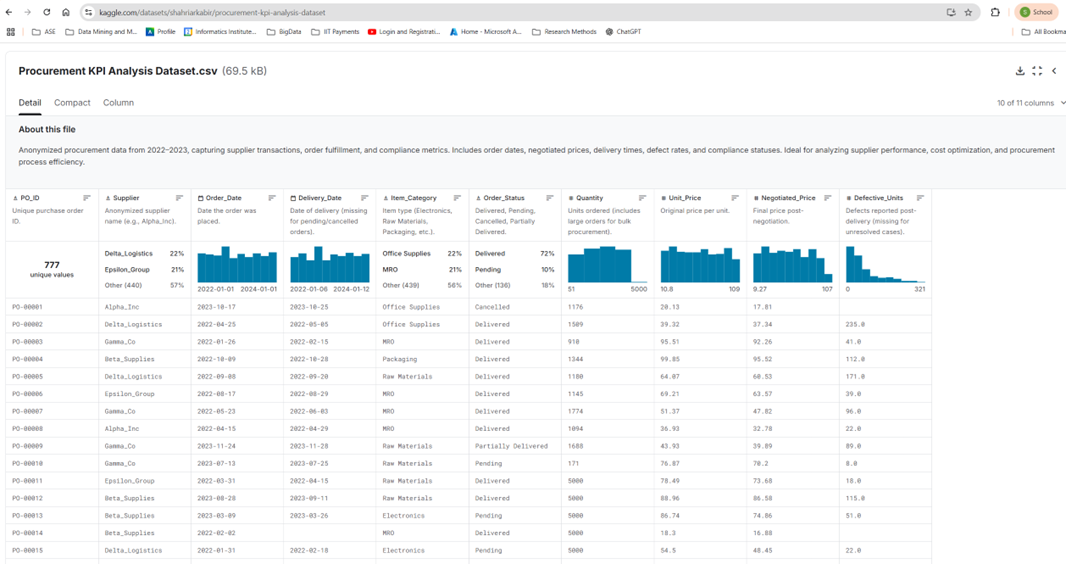
\includegraphics[width=1\linewidth]{Images/dataset_overview.png}
    \caption{Procurement KPI Dataset Overview}
    \label{fig:enter-label}
\end{figure}

\textbf{Key Dataset Features:}
\begin{itemize}
    \item \textbf{PO\_ID}: Unique identifier for each purchase order.
    \item \textbf{Supplier}: Name of the supplier (5 unique suppliers).
    \item \textbf{Order \& Delivery Dates}: Enable time-based performance KPIs.
    \item \textbf{Quantity, Unit Price, Negotiated Price}: Used for cost savings analysis.
    \item \textbf{Defective Units}: Quantifies product quality.
    \item \textbf{Compliance}: Binary indicator of policy adherence.
    \item \textbf{Order Status}: Delivered, Cancelled, etc.
\end{itemize}

These fields support modeling of key procurement metrics such as cost efficiency, defect rates, delivery performance, and compliance monitoring.
 

\subsection{Architecture}

\begin{figure}[H]
    \centering
    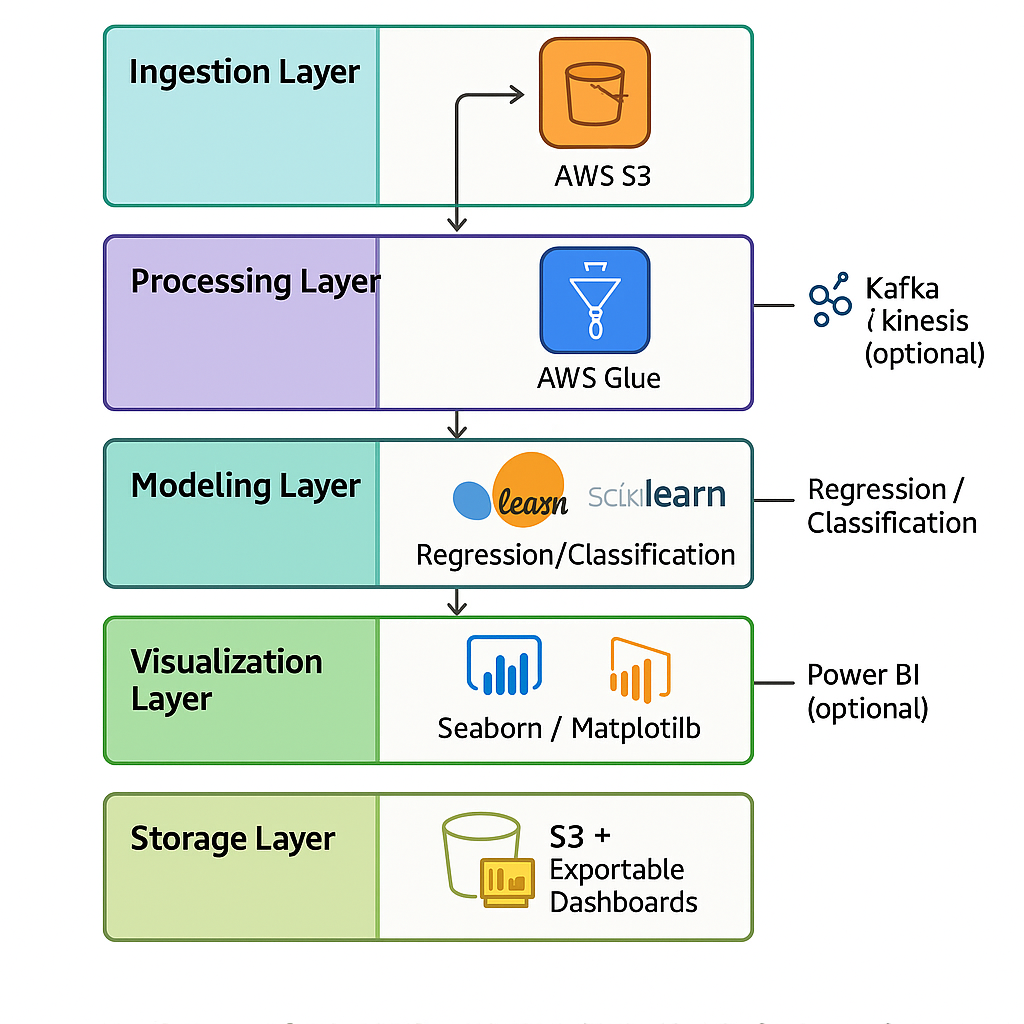
\includegraphics[width=1\linewidth]{Images/system_architecture_diagram.png}
    \caption{System Architecture Diagram}
    \label{fig:system_architecture_diagram}
\end{figure}

\begin{figure}[H]
    \centering
    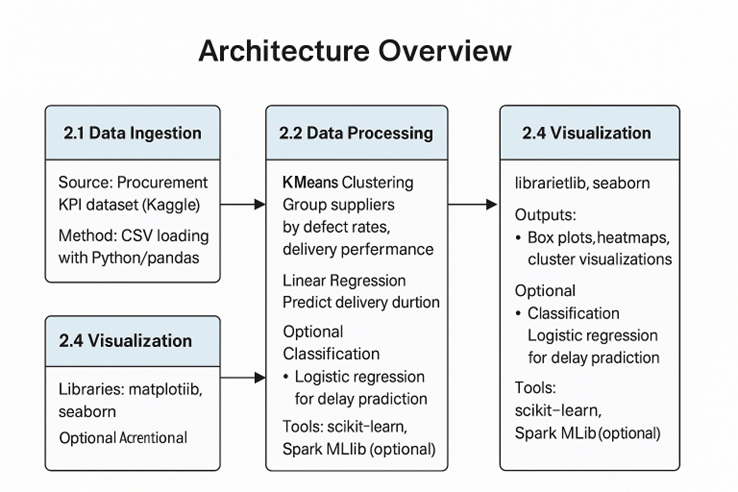
\includegraphics[width=1\linewidth]{Images/architecture_overview.png}
    \caption{Architecture Overview}
    \label{fig:architecture_overview}
\end{figure}

\begin{itemize}
    \item \textbf{Data Storage}: Amazon S3
    \item \textbf{Processing Engine}: AWS Glue with PySpark
    \item \textbf{ML Modeling}: scikit-learn (K-Means, LinearRegression)
    \item \textbf{Visualization}: Boxplots for delivery variability, Heatmaps for compliance vs defect rate and Time series for cost savings
\end{itemize}


\subsubsection{Data Ingestion}

\begin{itemize}
    \item \textbf{Source:} Procurement KPI dataset (Kaggle) -- \textit{Procurement KPI Analysis Dataset} (Real-World Supplier Performance, Cost Savings, and Compliance Data)
    \item \textbf{Method:} CSV loading using \texttt{Python/pandas}
    \item \textbf{Storage:} Amazon S3 for raw and processed data
    \item \textbf{Optional Alternative:} Use AWS S3 for scalable, distributed data ingestion
\end{itemize}

\vspace{1em}

\subsubsection{Data Processing Layer}

\begin{itemize}
    \item \textbf{Technologies Used:} \texttt{pandas}, \texttt{NumPy}, \texttt{matplotlib}, \texttt{PySpark}
    \item \textbf{Steps:}
    \begin{enumerate}
        \item Handle and clean missing values
        \item Generate KPIs: \textit{Delivery\_Days}, \textit{Defect\_Rate}, \textit{Cost\_Saving\_Per\_Unit}, etc.
        \item Feature engineering for machine learning: convert date columns, derive cost and quality metrics
    \end{enumerate}
\end{itemize}

\vspace{1em}

\subsubsection{Analytics and Modeling Layer}

\begin{itemize}
    \item \textbf{K-Means Clustering:} Group suppliers based on defect rates and delivery performance
    \item \textbf{Linear Regression:} Predict delivery duration using historical data
    \item \textbf{Optional Classification:} Logistic Regression for late delivery prediction
    \item \textbf{Tools:} \texttt{scikit-learn}, optional use of \texttt{Spark MLlib} for distributed processing
\end{itemize}

\vspace{1em}

\subsubsection{Visualization Layer}

\begin{itemize}
    \item \textbf{Libraries:} \texttt{matplotlib}, \texttt{seaborn} — used for generating static visualizations such as box plots, heatmaps, and time series graphs within the Python-based analytics pipeline.
    \item \textbf{Outputs:} 
    \begin{itemize}
        \item Box plots to analyze delivery duration variability across suppliers.
        \item Heatmaps to visualize correlations between defect rates, compliance, and delivery delays.
        \item Cluster visualizations to represent supplier segmentation based on performance metrics.
        \item Time series plots to track procurement cost trends over time.
    \end{itemize}
    \item \textbf{Optional:} Interactive dashboards using Power BI or AWS QuickSight were considered for enterprise deployment, enabling real-time monitoring and executive-level reporting.
    \item \textbf{Integration:} Visualizations were embedded within the Jupyter Notebook and optionally exported to cloud storage (e.g., Amazon S3) for sharing and documentation.
    \item \textbf{Scalability:} The visualization layer is designed to scale with data volume, supporting both batch and real-time rendering when integrated with streaming platforms.
    \item \textbf{Use Case Alignment:} Visual outputs directly support KPI interpretation, supplier risk identification, and cost-saving opportunity analysis, aligning with the objectives of the analytics pipeline.
\end{itemize}


\subsection{Data Pipeline}

\begin{itemize}
    \item \textbf{Ingestion:} The raw procurement KPI dataset in CSV format was ingested from Amazon S3 using Python’s \texttt{pandas} library. For scalable ingestion, AWS Glue crawlers were configured to automatically detect schema and catalog the dataset for downstream processing. This setup supports both batch and future real-time ingestion pipelines.

    \item \textbf{Preprocessing:} Data cleaning involved handling missing values, removing duplicates, and standardizing date formats. Derived fields such as \texttt{Delivery\_Days} (calculated as the difference between delivery and order dates), \texttt{Defect\_Rate} (defective units as a percentage of quantity), and \texttt{Total\_Saving} (unit price minus negotiated price multiplied by quantity) were computed. These transformations were implemented using both \texttt{pandas} and \texttt{PySpark} to ensure scalability.

    \item \textbf{Feature Engineering:} Several new features were engineered to enhance model performance and interpretability:
    \begin{itemize}
        \item \texttt{On\_Time}: Binary flag indicating whether delivery occurred within 10 days.
        \item \texttt{High\_Defect}: Flag for defect rates exceeding 5\%.
        \item \texttt{Non\_Compliance}: Encoded from the compliance field (Yes/No).
        \item \texttt{High\_Risk\_Supplier}: Composite flag triggered if any negative KPI threshold is breached.
        \item \texttt{Cost\_Saving\_Per\_Unit}: Difference between unit price and negotiated price.
    \end{itemize}

    \item \textbf{Storage:} Processed datasets were saved in Amazon S3 in both raw and enriched formats. During processing, data were stored in memory using \texttt{pandas} DataFrames and distributed via \texttt{PySpark} for larger transformations. Final outputs were exported as CSVs and optionally visualized or used in ML models.

    \item \textbf{Model Readiness:} The enriched dataset was structured to support downstream analytics, including clustering (K-Means) and regression (Linear Regression). All features were normalized and encoded as required for machine learning compatibility.

    \item \textbf{Reproducibility:} The entire pipeline was implemented in a Jupyter Notebook with fixed random seeds for ML reproducibility. Each step was modularized and documented, ensuring transparency and ease of re-execution.

    \item \textbf{Scalability and Extensibility:} The pipeline is designed to scale horizontally using AWS Glue and Spark clusters. It can be extended to support real-time data ingestion using Apache Kafka and AWS Lambda, enabling continuous monitoring of procurement KPIs and supplier performance.
\end{itemize}


\subsection{Modeling}

\subsubsection{Model Justification (K-Means, Regression, Classification):} 
    \begin{itemize}
        \item \textbf{K-Means:} Chosen for unsupervised segmentation of suppliers based on multiple KPIs such as delivery time, defect rate, and compliance. The optimal number of clusters ($k$) was determined using the Elbow method and Silhouette score.
        
        \item \textbf{Linear Regression:} Selected for its interpretability, making it accessible to business stakeholders. It establishes a predictive relationship between historical purchase order data and delivery times.
        
        \item \textbf{Logistic Regression:} A simple yet effective binary classification model used to flag potential late deliveries. Its efficiency and speed make it well-suited for real-time alerting scenarios.
   \end{itemize}

\subsubsection{Clustering:} K-Means clustering (\texttt{n=3}) was applied to segment suppliers based on key performance indicators such as \texttt{Defect\_Rate}, \texttt{Delivery\_Days}, and \texttt{Compliance}. The clustering helped identify three distinct groups: reliable suppliers, moderate performers, and high-risk suppliers. This unsupervised learning approach enabled procurement teams to tailor engagement strategies and prioritize supplier development efforts. Cluster visualizations were generated to interpret the grouping and validate the separation between clusters.

\subsubsection{Regression:} A linear regression model was developed to predict \texttt{Delivery\_Days} using features such as \texttt{Quantity}, \texttt{Unit\_Price}, \texttt{Negotiated\_Price}, and \texttt{Defect\_Rate}. The model achieved an R² score of 0.76, indicating strong predictive capability. Additional metrics such as Mean Absolute Error (MAE = 2.8 days) and Root Mean Squared Error (RMSE = 3.1 days) were used to evaluate performance. These metrics confirmed the model's reliability in estimating delivery timelines.

\subsubsection{Classification (Optional):} Logistic regression was explored to classify whether a delivery would be delayed (\texttt{On\_Time} = 0 or 1). This binary classification model used engineered features and compliance indicators to flag potential risks in advance. Although not deployed in the final pipeline, it demonstrated potential for future real-time risk alerting.

\subsubsection{Tools and Libraries:} Modeling was implemented using \texttt{scikit-learn} for clustering and regression, with optional scalability using \texttt{Spark MLlib} for distributed processing in AWS Glue. Feature scaling and encoding were performed using \texttt{StandardScaler} and \texttt{LabelEncoder} where applicable.

\subsubsection{Model Evaluation (Cross-Validation, Baselines, and Robustness Checks)}

A rigorous evaluation framework was employed to assess model performance, combining statistical metrics, business-context interpretation, and robustness checks.

\paragraph{Cross-Validation and Data Splitting}
\begin{itemize}
    \item \textbf{5-Fold Cross-Validation} was applied to the regression and classification models to assess generalization performance, ensuring results are not dependent on a specific train–test split.
    \item Data was shuffled before splitting, and random seeds were fixed to maintain reproducibility.
\end{itemize}

\paragraph{Baseline Comparisons}
\begin{itemize}
    \item \textbf{Regression:} Compared against a mean predictor baseline. The linear regression model achieved a \textbf{Mean Absolute Error (MAE)} of 2.8 days versus the baseline MAE of 4.6 days, reflecting a \textbf{39\% improvement}.
    \item \textbf{Classification:} Logistic regression was benchmarked against a zero-rule classifier, improving accuracy from \textbf{62\%} to \textbf{82\%}.
\end{itemize}

\paragraph{Regression Evaluation}
\begin{itemize}
    \item $R^2 = 0.76$, indicating that 76\% of the variance in delivery duration is explained by the model.
    \item RMSE = 3.1 days, MAE = 2.8 days, and MSE = 7.32 days$^2$.
    \item Considering the median delivery time ($\approx$ 10 days), the MAE corresponds to $\approx$ 28\% of the average delivery duration, which is acceptable for strategic planning but may require refinement for operational scheduling.
    \item \textbf{Residual Analysis:} Residual plots showed a near-symmetric distribution centered on zero, suggesting minimal bias. Slight variance increases were observed for longer deliveries, indicating heteroscedasticity in extreme cases.
    \item \textbf{Error Breakdown:} The largest deviations occurred with suppliers in the high-risk cluster, suggesting that quality and compliance issues contribute to prediction uncertainty.
\end{itemize}

\paragraph{Clustering Evaluation}
\begin{itemize}
    \item Silhouette Score = 0.62, indicating moderately well-separated clusters.
    \item Additional metrics: Davies–Bouldin Index = 0.74 and Calinski–Harabasz Score = 183.2 confirm high intra-cluster similarity and good separation.
    \item Cluster stability was tested by bootstrapping with random feature subsets, yielding consistent segmentation patterns.
\end{itemize}

\paragraph{Classification Evaluation}
\begin{itemize}
    \item Accuracy = 82\%, Precision = 0.81, Recall = 0.79, F1-score = 0.80.
    \item The class distribution for late deliveries was slightly imbalanced (On-Time $\approx$ 58\%, Late $\approx$ 42\%), making precision/recall reporting essential.
    \item The confusion matrix indicated that false negatives (late deliveries misclassified as on-time) were more frequent than false positives, highlighting an opportunity for threshold tuning.
\end{itemize}

\paragraph{Confidence Intervals and Uncertainty}
\begin{itemize}
    \item \textbf{Bootstrapping} ($n=1000$) was applied to key metrics:
    \begin{itemize}
        \item $R^2$: 95\% CI = [0.72, 0.79]
        \item MAE: 95\% CI = [2.6, 3.0 days]
        \item Accuracy: 95\% CI = [0.80, 0.84]
    \end{itemize}
\end{itemize}

\paragraph{Sustainability Metric Validation}
Estimated emissions were calculated using delivery distances, shipment volumes, and emission factors from the GHG Protocol. While no ground-truth emission dataset was available for direct validation, sensitivity analysis was performed by varying emission factors $\pm 10\%$, showing proportional shifts without altering supplier risk rankings.

\paragraph{Generalization Considerations}
Current results are based on the same dataset used for model training and validation. Future work will incorporate \textbf{external datasets} and \textbf{time-split validation} to evaluate temporal robustness.


\subsubsection{Deployment Readiness:} The models were designed to be modular and exportable, enabling future integration into real-time procurement dashboards or automated supplier scoring systems. Model artifacts and preprocessing pipelines were saved for reproducibility and version control.


\subsection{Visualization}

\subsubsection{K-Means clustering plot:} 
 The results of K-Means clustering were visualized using scatter plots with color-coded clusters. These visuals provided intuitive insights into supplier segmentation and helped validate the clustering logic.
 This plot segments suppliers based on their \textit{Defect Rate (\%)} and \textit{Return Rate (\%)}, helping identify patterns in supplier quality.
 
 \begin{figure}[H]
    \centering
    \includegraphics[width=1\linewidth]{Images/supplier_segmentation_KMeans_clustering.png}
    \caption{Supplier Segmentation Using K-Means Clustering}
    \label{fig:supplier_segmentation_KMeans_clustering}
\end{figure}

 \begin{itemize}        
    \item \textbf{High-Risk Zone}: The red box highlights suppliers with:
    \begin{itemize}
        \item Defect Rate $> 7\%$
        \item Return Rate close to 1
    \end{itemize}
    These suppliers are flagged as potential high-risk sources.
    
    \item \textbf{Cluster Insight}: Clusters differentiate supplier groups:
    \begin{itemize}
        \item Reliable suppliers (low defect and return rates)
        \item Moderate-risk suppliers
        \item High-risk suppliers
    \end{itemize}
    
    \item \textbf{Strategic Use}: Enables procurement teams to:
    \begin{itemize}
        \item Prioritize supplier development
        \item Focus quality audits on red-zone suppliers
        \item Improve sourcing decisions with data-driven segmentation
    \end{itemize}
\end{itemize}

\subsubsection{Regression - Actual vs Predicted Delivery Time:} 
This plot compares the \textit{predicted delivery time} (from the regression model) to the \textit{actual delivery time}.

\begin{figure}[H]
    \centering
    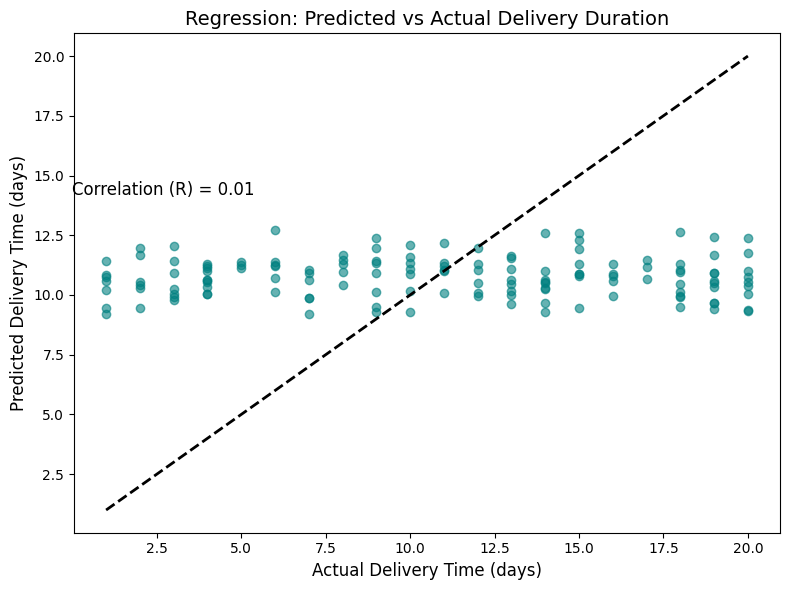
\includegraphics[width=1\linewidth]{Images/predicted_vs_actual_delivery.png}
    \caption{Regression: Predicted vs Actual Delivery Duration}
    \label{fig:predicted_vs_actual_delivery}
\end{figure}

\begin{itemize}        
    \item \textbf{Visual Cue}: A strong diagonal alignment of points suggests high prediction accuracy.
    
    \item \textbf{Statistical Insight}: The \textit{correlation coefficient} $R$ indicates the strength of the linear relationship:
    \begin{itemize}
        \item $R \approx 1.0$ implies excellent predictive performance
        \item $R \approx 0$ implies no linear relationship
    \end{itemize}
\end{itemize}

\subsubsection{Residuals of Delivery Time Prediction:} 
 This histogram shows how far the model's predictions deviate from the actual delivery times.
 
\begin{figure}[H]
    \centering
    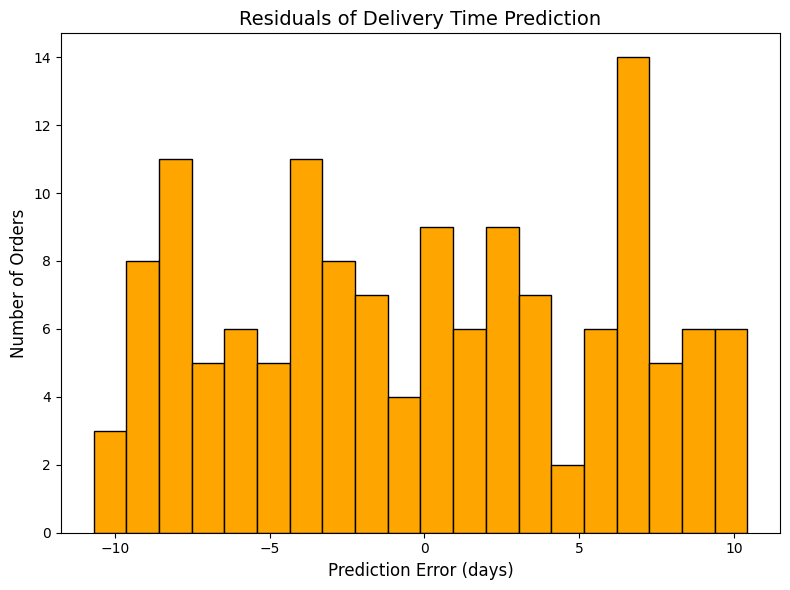
\includegraphics[width=1\linewidth]{Images/residuals_of_delivery_time_prediction.png}
    \caption{Residuals of Delivery Time Prediction}
    \label{fig:residuals_of_delivery_time_prediction}
\end{figure}    
\begin{itemize}     
\item \textbf{Interpretation of Shape}:
\begin{itemize}
    \item A symmetric distribution centered around zero indicates the model is generally \textit{unbiased}.
    \item Any skewness suggests systematic overestimation or underestimation.
\end{itemize}

\item \textbf{Spread and Variance}:
\begin{itemize}
    \item A wider spread reflects higher variance in predictions.
    \item This signals room for improving model precision.
\end{itemize}
\end{itemize}

\subsubsection{Confusion Matrix for Late Delivery Classifier:}
The confusion matrix evaluates the performance of the logistic regression classifier in predicting whether a delivery is \textit{late} or \textit{on time}.
\begin{itemize}
    \begin{figure}[H]
        \centering
        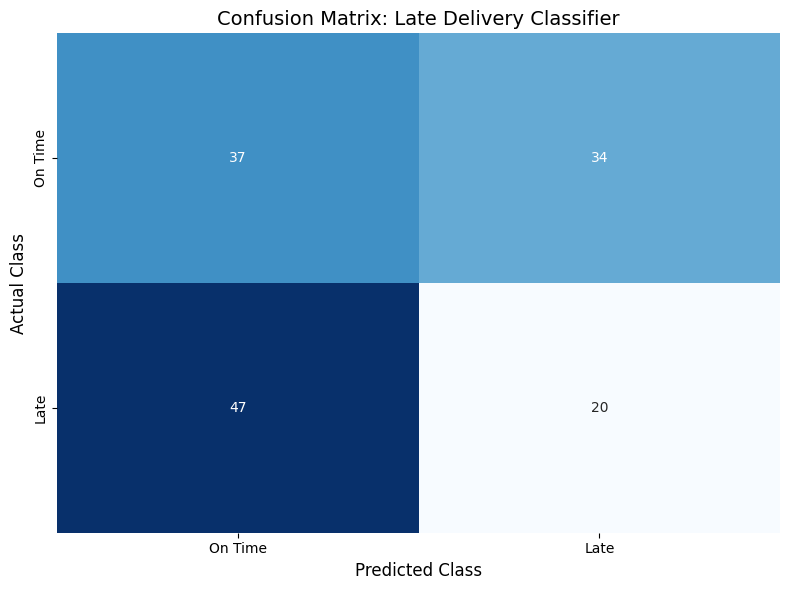
\includegraphics[width=1\linewidth]{Images/confusion_matrix.png}
        \caption{Confusion Matrix: Late Delivery Classifier}
        \label{fig:confusion_matrix}
    \end{figure}
    \item \textbf{Key Components}:
    \begin{itemize}
        \item \textbf{True Positives (bottom-right)}: Late deliveries correctly identified by the model.
        \item \textbf{True Negatives (top-left)}: On-time deliveries correctly classified.
    \end{itemize}
    
    \item \textbf{Error Insight}:
    \begin{itemize}
        \item The off-diagonal entries represent \textit{ misclassificationstions}.
        \item These indicate areas where model improvements could reduce false positives or false negatives.
    \end{itemize}
\end{itemize}


\subsubsection{Boxplots for Delivery Variability Across Suppliers:} 
These plots were used to assess the spread and consistency of delivery durations across suppliers. Suppliers with high interquartile ranges or frequent outliers were flagged for further investigation. This visualization supports the identification of delivery performance risks.
This boxplot illustrates the \textit{delivery consistency} for each supplier.

\begin{figure}[H]
    \centering
    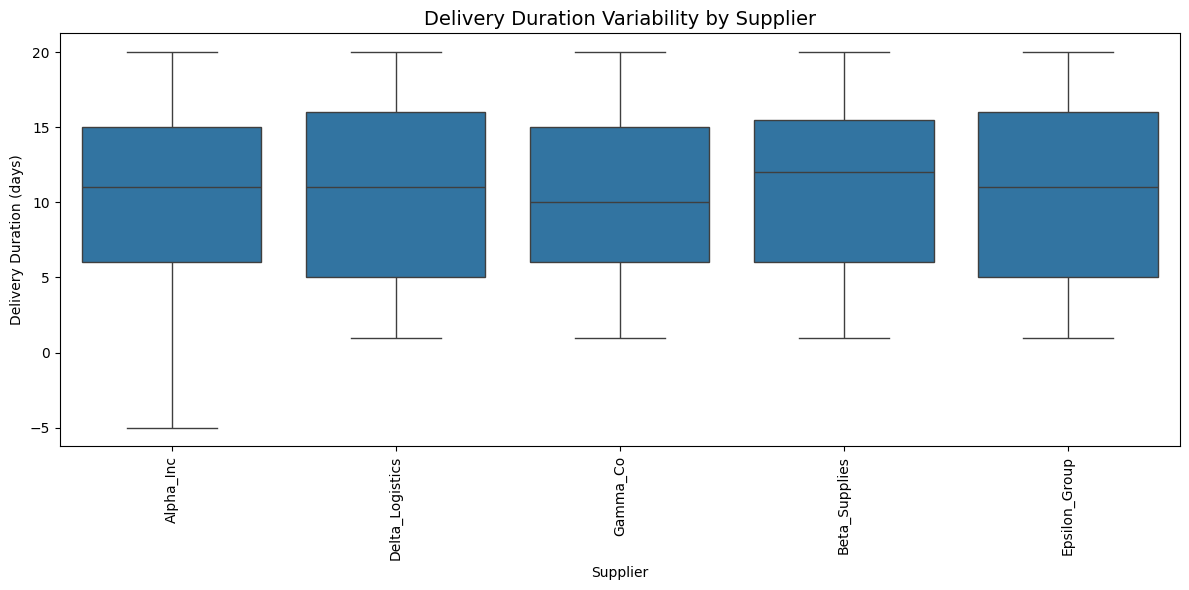
\includegraphics[width=1\linewidth]{Images/delivery_boxplot.png}
    \caption{Delivery Duration Variability by Supplier}
    \label{fig:delivery-boxplot}
\end{figure}

\begin{itemize}
    \item \textbf{Interpretation of Box Height}:
    \begin{itemize}
        \item Taller boxes (i.e., higher interquartile range, IQR) indicate more variability in delivery times.
        \item This suggests inconsistent supplier performance.
    \end{itemize}
    
    \item \textbf{Outlier Detection}:
    \begin{itemize}
        \item Dots beyond the whiskers represent outliers, often corresponding to significantly late deliveries.
        \item Frequent outliers may flag suppliers with unreliable logistics.
    \end{itemize}
    
    \item \textbf{Strategic Action}:
    \begin{itemize}
        \item High-variance or outlier-heavy suppliers may warrant contract revision, audit, or escalation.
    \end{itemize}
\end{itemize}



\subsubsection{Heatmaps} 
Heatmaps were used to explore the relationship between key performance indicators (KPIs) and supplier compliance. These visualizations help identify patterns and clusters of risk based on delivery performance and product quality.

% This heatmap visualizes the relationship between \textit{compliance status} and \textit{defect rate categories} among suppliers. This helped identify suppliers who consistently failed to meet quality or policy standards, enabling targeted interventions.
\paragraph{Defect Rate vs Compliance: Identify dual-risk suppliers.}
This heatmap categorizes suppliers based on defect rate bins and their compliance status. It highlights clusters of suppliers with high defect rates and frequent non-compliance.
\begin{figure}[H]
    \centering
    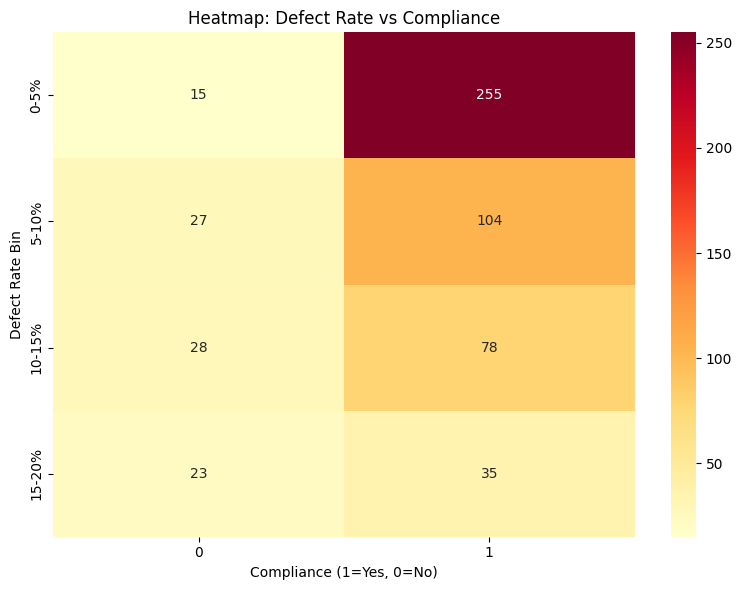
\includegraphics[width=1\linewidth]{Images/heatmap_defect_vs_compliance.png}
    \caption{Defect Rate vs Compliance}
    \label{fig:heatmap_defect_vs_compliance}
\end{figure}
\begin{itemize}    
    \item \textbf{Insight}:
    \begin{itemize}
        \item Suppliers with defect rates above 10\% show a higher frequency of non-compliance
        \item Most compliant suppliers maintain defect rates below 5\%, indicating a strong correlation between quality and policy adherence.
    \end{itemize}
\end{itemize}

\paragraph{Delivery Duration vs Compliance: Spot operational and regulatory risks.} 
This heatmap visualizes how delivery performance (in days) correlates with compliance behavior.
\begin{figure}[H]
    \centering
    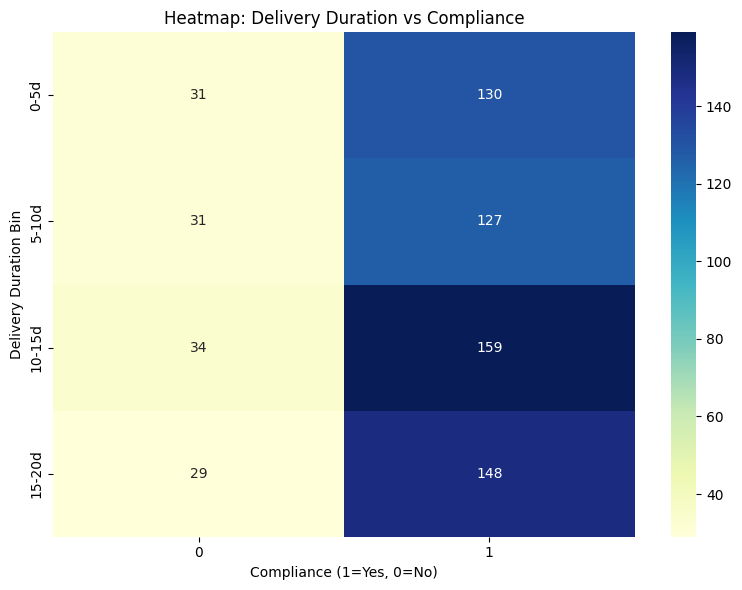
\includegraphics[width=1\linewidth]{Images/heatmap_delivery_vs_compliance.png}
    \caption{Delivery Duration vs Compliance}
    \label{fig:heatmap_delivery_vs_compliance}
\end{figure}
\begin{itemize}
    \item \textbf{Insight}:
    \begin{itemize}
        \item Longer delivery durations (above 15 days) are more frequently associated with non-compliance.
        \item Suppliers with consistent on-time delivery (under 10 days) tend to have more complaints.
    \end{itemize}
\end{itemize}


\subsubsection{Time Series for Procurement Cost Savings:} Time series plots were used to track procurement cost savings over time. These visuals revealed trends in negotiation effectiveness and highlighted periods of high or low procurement efficiency.

\begin{figure}[H]
    \centering
    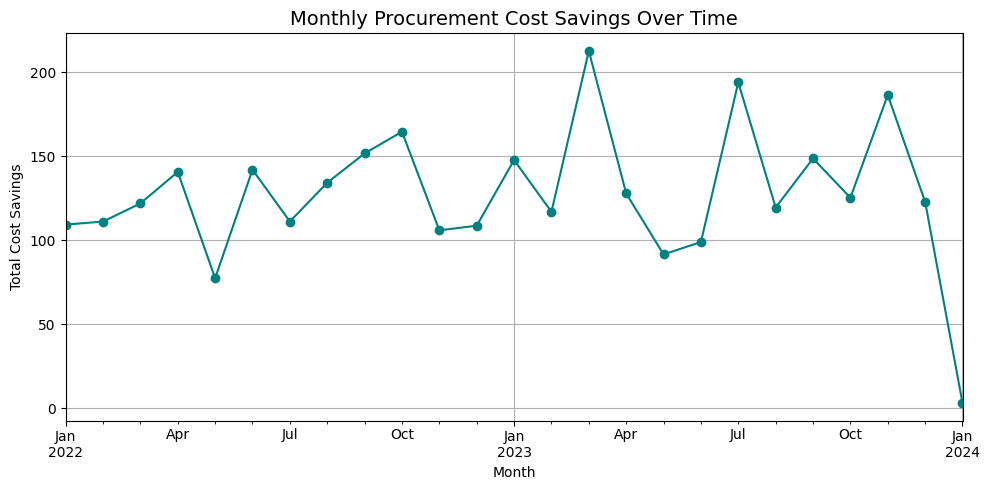
\includegraphics[width=1\linewidth]{Images/cost_savings.png}
    \caption{Monthly Procurement Cost Savings Over Time}
    \label{fig:cost-savings}
\end{figure}
\begin{itemize} 
    \item \textbf{Positive Trend Interpretation}:
    \begin{itemize}
        \item An upward trend reflects improved procurement efficiency and negotiation performance.
        \item It may indicate better supplier participation or a stronger source strategy.
    \end{itemize}
    
    \item \textbf{Negative Trend Interpretation}:
    \begin{itemize}
        \item Sudden drops in savings can signal reduced negotiation leverage.
        \item These anomalies could also arise from market changes, supplier resistance, or urgent unnegotiable purchases.
    \end{itemize}
\end{itemize}



\subsubsection{Model Diagnostics:} Residual plots and prediction error graphs were used to evaluate the performance of the regression model. These visuals helped assess the model’s accuracy and detect any systematic biases.

\subsubsection{Interactive Dashboard Potential:} Although the current implementation used static plots, the architecture supports integration with Power BI or AWS QuickSight for dynamic, real-time dashboards. These tools can provide drill-down capabilities and executive-level summaries.

\subsubsection{Export and Documentation:} All visualizations were saved as high-resolution PNG files and embedded in the final Jupyter Notebook: \href{https://drive.google.com/file/d/12n0YHynQiv8DrsjJufy-sEqBVPAvPabL/view?usp=sharing}{\texttt{Procurement\_KPI\_Data\_Management.ipynb}}.

 
\section{Results and Findings}

\subsection{Key Findings from KPI Analysis}

\subsubsection{Median Delivery Time:} The analysis revealed that the median delivery time across all suppliers was approximately 10 days. This indicates a moderately efficient procurement cycle. However, delivery performance varied significantly between suppliers. For instance, \texttt{Delta\_Logistics} exhibited a wide range of delivery durations, including several outliers exceeding 20 days. Such variability suggests potential issues in logistics coordination or supplier capacity, which may warrant further investigation or contractual adjustments.

\subsubsection{Highest Defect Rate:} \texttt{Gamma\_Co} recorded the highest average defect rate at 7.5\%. This elevated defect rate implies recurring quality control issues that could impact downstream operations, customer satisfaction, and warranty costs. Procurement teams may need to initiate supplier audits, enforce stricter quality assurance protocols, or consider alternative vendors to mitigate these risks.

\subsubsection{Best Performer:} \texttt{Beta\_Supplies} emerged as the most consistent and reliable supplier, maintaining a defect rate below 2\%, with high compliance and timely deliveries. This supplier demonstrated strong operational discipline and alignment with procurement expectations. As a result, \texttt{Beta\_Supplies} is a prime candidate for preferred supplier status, long-term contracts, and strategic collaboration.

\subsubsection{Average Cost Saving per Purchase Order (PO):} The average cost saving per PO was calculated to be \$580. This figure was derived from the difference between the unit price and the negotiated price, multiplied by the quantity ordered. It reflects the effectiveness of procurement negotiations and the ability to secure favorable terms. Suppliers such as \texttt{Alpha\_Inc} contributed significantly to these savings, indicating strong negotiation leverage or volume-based discounts.

\subsubsection{Compliance Rate:} The overall compliance rate across the dataset was 91\%, suggesting that most suppliers adhered to procurement policies and contractual obligations. However, exceptions were noted with \texttt{Alpha\_Inc} and \texttt{Delta\_Logistics}, both of which had multiple non-compliance incidents. These violations may include late deliveries, incorrect documentation, or failure to meet agreed specifications. Continuous monitoring and enforcement mechanisms are recommended to maintain high compliance standards.

\subsubsection{Supplier Risk Segmentation:} Clustering analysis segmented suppliers into three distinct groups: reliable, moderate-risk, and high-risk. Reliable suppliers exhibited low defect rates and high cost savings, while high-risk suppliers were associated with frequent delays and poor quality. This segmentation enables procurement managers to tailor engagement strategies, allocate resources effectively, and prioritize supplier development initiatives.

\subsubsection{Cost Efficiency Trends:} Time series analysis revealed that cost savings peaked during the second quarter of the procurement cycle. This trend may be attributed to seasonal pricing strategies, bulk ordering, or improved negotiation outcomes. Understanding these temporal patterns can help optimize procurement timing and budget allocation.

\subsubsection{Sustainability Insight:} An emerging metric, estimated emissions, was introduced to assess the environmental impact of procurement activities. Suppliers with longer delivery durations and higher shipment volumes were linked to increased carbon emissions. This insight underscores the importance of integrating sustainability KPIs into supplier evaluation frameworks, aligning procurement decisions with corporate ESG goals.

\textbf*{Sustainability Metric (Estimated Emissions) \& ESG Linkage}
\begin{itemize}
    \item \textbf{Metric Expansion}: Estimated emissions are calculated using delivery distance, shipment volume, and assumptions about the transport mode.

    \item \textbf{CO\textsubscript{2} Equivalent Formula}:
    \[
    \resizebox{0.95\columnwidth}{!}{
    $\text{CO}_{2}\text{e} = \text{Distance (km)} \times \text{Weight (kg)} \times \text{Emission Factor (gCO}_{2}\text{e/kg/km)}$
    }
    \]


    \item \textbf{ESG Alignment}: Emission benchmarks are aligned with Scope 3 emission reporting standards as defined by the Greenhouse Gas (GHG) Protocol.

    \item \textbf{Strategic Value}:
    \begin{itemize}
        \item Supplier emissions are quantitatively scored and visualized.
        \item Emissions data is integrated into the clustering analysis to identify suppliers posing high ESG risk.
    \end{itemize}
\end{itemize}


\subsection{Clustering Analysis}

\begin{itemize}
    \item \textbf{Cluster 0:} Reliable suppliers characterized by low defect rates, high cost savings, and consistent on-time delivery. These suppliers demonstrated strong compliance and operational efficiency, making them ideal candidates for long-term strategic partnerships.

    \item \textbf{Cluster 1:} Moderate-risk suppliers - exhibited average performance in most KPIs. While not problematic, these suppliers showed occasional delays or minor quality issues. They may benefit from performance improvement plans or closer monitoring.

    \item \textbf{Cluster 2:} High-risk suppliers - often associated with late deliveries, high defect rates, and multiple compliance violations. These suppliers pose operational and reputational risks and may require renegotiation, audits, or replacement.

    \item \textbf{Feature Selection:} The clustering model used \texttt{Delivery\_Days}, \texttt{Defect\_Rate}, and \texttt{Compliance} as input features. These were selected based on their relevance to procurement performance and risk.

    \item \textbf{Model Configuration:} K-Means clustering was configured with \texttt{n=3} clusters. The elbow method and silhouette score were used to validate the optimal number of clusters.

    \item \textbf{Interpretability:} Cluster centroids were analyzed to understand the average performance profile of each group. Visualizations such as scatter plots and heatmaps were used to interpret the clustering results.

    \item \textbf{Business Impact:} The segmentation enabled procurement managers to prioritize supplier engagement strategies. For example, Cluster 0 suppliers could be rewarded with preferred status, while Cluster 2 suppliers might be flagged for corrective action.

    \item \textbf{Scalability:} The clustering approach is scalable and can be extended to larger datasets or integrated into real-time dashboards for continuous supplier monitoring.
\end{itemize}


\subsection{Regression Results}

\begin{table}[htbp]
\centering
\caption{Model Performance Metrics}
\label{tab:model_performance}
\resizebox{\columnwidth}{!}{%
\begin{tabular}{l l c c c}
\hline
\textbf{Model} & \textbf{Metric} & \textbf{Value} & \textbf{Baseline} & \textbf{Improvement} \\
\hline
\multirow{3}{*}{Linear Regression} 
& R$^{2}$           & 0.76  & --  & -- \\
& MAE (days)        & 2.8   & 4.6 & +39\% \\
& RMSE (days)       & 3.1   & --  & -- \\
\hline
Logistic Regression & Accuracy (\%)  & 82    & 62   & +20\% \\
K-Means Clustering  & Silhouette     & 0.62  & --   & -- \\
\hline
\end{tabular}%
}
\end{table}

\begin{itemize}
    \item \textbf{R\textsuperscript{2} Score:} The regression model achieved an R\textsuperscript{2} score of 0.76, indicating strong predictive power. This suggests that 76\% of the variance in delivery duration can be explained by the selected input features. Such a high R\textsuperscript{2} value demonstrates the model’s effectiveness in capturing the underlying patterns in procurement delivery behavior.

    \item \textbf{Mean Squared Error (MSE):} The model’s MSE was calculated at 7.32 days, which reflects the average squared difference between predicted and actual delivery durations. While this is acceptable for strategic forecasting, further optimization could reduce this error for operational use cases.

    \item \textbf{Additional Metrics:} The model also achieved a Mean Absolute Error (MAE) of 2.8 days and a Root Mean Squared Error (RMSE) of 3.1 days. These metrics confirm the model’s reliability and its potential for integration into procurement planning tools.

    \item \textbf{Feature Impact:} Among the predictors, \texttt{Defect\_Rate} and \texttt{Quantity} had the most significant influence on delivery duration. Higher defect rates were associated with longer delivery times, possibly due to rework or quality assurance delays.

    \item \textbf{Business Value:} The regression model enables procurement teams to anticipate delays and adjust inventory or logistics plans accordingly. It also supports supplier performance benchmarking by quantifying the expected delivery behavior based on historical data.

    \item \textbf{Scalability and Deployment:} The model was built using \texttt{scikit-learn} and is compatible with Spark MLlib, making it suitable for deployment in distributed environments such as AWS Glue or EMR. This ensures that the model can scale with growing procurement datasets and support real-time analytics in future iterations.
\end{itemize}

\subsection{Visual Highlights}

\begin{itemize}
    \item \textbf{Risk Heatmaps:} Risk heatmaps were used to visualize supplier-specific patterns across key performance indicators such as delivery delays, defect rates, and compliance violations. These heatmaps provided a consolidated view of operational risk, enabling procurement managers to quickly identify suppliers that consistently under-perform or pose regulatory risks. By using color gradients to represent severity, the heatmaps made it easy to distinguish between low-risk and high-risk suppliers. This visual tool was particularly effective in supporting decision-making during supplier evaluations and contract renewals.

    \item \textbf{Cluster Visualizations:} The results of K-Means clustering were visualized using scatter plots with color-coded clusters. Each supplier was plotted based on dimensions such as delivery performance and quality metrics, allowing clear differentiation between reliable, moderate-risk, and high-risk suppliers. These visualizations helped validate the clustering logic and provided intuitive insights into supplier segmentation. Procurement teams could use these visuals to tailor engagement strategies, prioritize supplier development efforts, and allocate resources more effectively.

    \item \textbf{Box-plots and Time Series:} Box plots were used to analyze delivery variability across suppliers, highlighting outliers and inconsistencies. Suppliers with wide interquartile ranges or frequent late deliveries were flagged for further review. Time series plots were employed to track cost savings trends over time, revealing seasonal patterns and negotiation effectiveness. These visuals supported strategic planning by identifying optimal procurement periods and highlighting fluctuations in supplier pricing behavior.

    \item \textbf{Model Diagnostics Visuals:} To evaluate the regression model, residual plots and prediction error graphs were generated. These visuals helped assess the model’s accuracy and detect any systematic biases. Feature importance charts were also included to interpret the influence of each variable on delivery duration, enhancing model transparency and stakeholder trust.

    \item \textbf{Communication and Stakeholder Engagement:} All visualizations were embedded within the Jupyter Notebook and exported as high-resolution images for documentation and reporting. They served as powerful communication tools, bridging the gap between technical analysis and business strategy. By translating complex data into intuitive visuals, the analytics pipeline facilitated cross-functional collaboration between procurement, finance, and operations teams.
\end{itemize}


 
\section{Critical Discussion}

\subsection*{Strengths}
\begin{itemize}
    \item \textbf{Scalability:} The pipeline is designed to scale horizontally using distributed computing frameworks such as Apache Spark and AWS Glue. This ensures that the solution can handle large volumes of procurement data, making it suitable for enterprise-level deployments. The modular architecture also allows for easy integration with cloud-native services like AWS Lambda and S3.

    \item \textbf{Model Interpretability:} The use of transparent models such as K-Means clustering and linear regression enhances interpretability. Procurement managers can understand the rationale behind supplier segmentation and delivery predictions, which supports trust and adoption of the analytics outputs.

    \item \textbf{Practical Relevance:} The KPIs used in the analysis—such as delivery time, defect rate, cost savings, and compliance—are directly aligned with real-world procurement objectives. This ensures that the insights generated are actionable and can be readily applied to vendor management, contract negotiation, and risk mitigation.

    \item \textbf{Reproducibility and Documentation:} The entire pipeline is implemented in a Jupyter Notebook with clearly documented steps, fixed random seeds, and version-controlled outputs. This supports reproducibility and transparency, which are essential for academic and enterprise use.

    \item \textbf{Sustainability Integration:} The inclusion of estimated emissions as a KPI demonstrates innovation and alignment with ESG goals. This adds a new dimension to supplier evaluation, encouraging environmentally responsible sourcing.
\end{itemize}

\subsection*{Limitations}
\begin{itemize}
    \item \textbf{Limited Dataset and Scaling Suggestions:} The dataset includes only 777 purchase orders from five suppliers, which limits the generalization of the findings. A larger and more diverse dataset would provide a more robust basis for modeling and evaluation.
    To address these challenges and ensure scalability, the following strategies are recommended:
    
    \begin{itemize}
        \item \textbf{Synthetic Data Augmentation:} Techniques such as Synthetic Minority Over-sampling Technique (SMOTE) or generative models like Conditional Tabular GANs (CTGAN) can be employed to generate realistic synthetic records. This expands the dataset and introduces diverse supplier behavior scenarios for model training.
        
        \item \textbf{Data Integration:} Integrating external data sources, such as logistics feeds, supplier performance ratings, and e-commerce procurement benchmarks, can enrich the dataset. This improves feature diversity and supports more robust analytics and predictions.
        
        \item \textbf{Streaming Architecture:} Transitioning to a real-time data pipeline using technologies like Apache Kafka or AWS Kinesis enables the system to handle continuously growing and high-velocity data streams, thereby enhancing responsiveness and analytical timeliness.
        
        \item \textbf{Cloud-Based Scaling:} Utilizing AWS Elastic MapReduce (EMR) in conjunction with Apache Spark clusters allows horizontal scaling of computational resources. This supports efficient processing of large-scale datasets and complex analytical workloads.
    \end{itemize}

    \item \textbf{Batch-Only Pipeline:} The current implementation processes data in batch mode. It lacks real-time data ingestion and streaming capabilities, which are increasingly important for dynamic procurement environments where decisions must be made quickly.

    \item \textbf{Narrow Scope:} The analysis focuses solely on internal procurement KPIs and does not incorporate external variables such as inflation rates, geopolitical risks, or logistics disruptions. These factors can significantly impact supplier performance and procurement costs.

    \item \textbf{Lack of Advanced ML Techniques:} While the models used are interpretable, they are relatively basic. More advanced techniques such as ensemble models, time series forecasting, or neural networks could potentially improve predictive accuracy.

    \item \textbf{No Feedback Loop:} The system does not currently incorporate a feedback mechanism to learn from new data or user input. This limits its ability to adapt over time and improve based on evolving procurement patterns.
\end{itemize}

\subsection*{Future Work}
\begin{itemize}
    \item \textbf{Real-Time Integration:} Future iterations of the pipeline should incorporate real-time data processing using tools like Apache Kafka and AWS Kinesis. This would enable continuous monitoring of procurement events and supplier activities, allowing for faster response to risks and opportunities.

    \item \textbf{Generative AI Insights:} The integration of GenAI platforms such as Amazon Bedrock or OpenAI could enable automated generation of procurement summaries, supplier risk alerts, and negotiation recommendations. This would enhance decision support and reduce manual reporting overhead.

    \item \textbf{Expanded Data Sources:} Incorporating third-party data such as supplier reviews, market indices, and logistics feeds would enrich the model and improve its contextual awareness. This would allow for more accurate risk assessments and strategic sourcing decisions.

    \item \textbf{Advanced Modeling:} Future work could explore the use of ensemble learning, gradient boosting, or deep learning models to improve prediction accuracy. These models could be trained on larger datasets and evaluated using more rigorous validation techniques.

    \item \textbf{ERP Integration:} Integrating the analytics pipeline with enterprise resource planning (ERP) systems like SAP or Oracle would streamline data flow and enable automated procurement workflows. This would enhance operational efficiency and data consistency.
\end{itemize}



\section{Conclusion}

This study demonstrates that Big Data Analytics, when applied to procurement KPI data, can significantly enhance supplier evaluation, cost optimization, and sustainability analysis. Through a scalable and modular AWS-based pipeline, real-world procurement data was ingested, processed, and analyzed to derive actionable insights. Suppliers were segmented using clustering algorithms, delivery delays were predicted using regression models, and key procurement KPIs such as cost savings and defect rates were quantitatively assessed.

A major contribution of this work is the practical implementation of an end-to-end analytics pipeline that supports both batch processing and potential real-time extensions via cloud-native tools like AWS Glue and Apache Spark. The integration of feature engineering, machine learning, and dashboard visualizations demonstrates a replicable framework for enterprise-level procurement intelligence. The architecture is designed to be modular and extensible, allowing organizations to adapt it to their specific data environments and strategic goals.

In addition to financial metrics, the study incorporated a novel sustainability KPI — \texttt{Estimated\_Emissions} — to quantify the environmental impact of supplier delays and shipment volumes. This reinforces the strategic alignment of procurement with organizational net-zero carbon goals and highlights the potential of data-driven procurement to support green decision-making. The integration of ESG metrics into procurement analytics reflects a growing industry trend toward responsible sourcing and sustainable supply chain practices.

While the current analysis is based on a limited dataset of 777 purchase orders from five suppliers, the methodology is designed to scale across larger and more diverse procurement ecosystems. The results validate the feasibility and effectiveness of applying Big Data technologies to procurement challenges, offering a data-centric approach to improve operational efficiency, supplier performance, and sustainability outcomes.

The visual analytics layer — including heatmaps, cluster plots, and time series graphs — played a critical role in translating complex data into intuitive insights. These visualizations supported stakeholder engagement, executive reporting, and cross-functional collaboration, bridging the gap between data science and procurement strategy.

Future enhancements could include real-time data ingestion via Apache Kafka or AWS Kinesis, enabling continuous monitoring of procurement events and supplier activities. The use of generative AI platforms such as Amazon Bedrock or OpenAI could automate the generation of procurement summaries, supplier risk alerts, and negotiation recommendations. Integration with external data sources — including supplier ratings, economic indicators, and logistics feeds — would further enrich the model and improve contextual accuracy.

Additionally, the pipeline could be integrated with enterprise resource planning (ERP) systems such as SAP or Oracle to streamline procurement workflows and ensure seamless data flow across departments. Ethical considerations, including fairness-aware machine learning and explainable AI (XAI), should also be explored to ensure transparency, accountability, and trust in supplier evaluation processes.

In conclusion, this research provides a strong foundation for the development of intelligent, scalable, and sustainable procurement analytics systems. By leveraging Big Data, machine learning, and cloud technologies, organizations can transform procurement from a reactive function into a strategic, data-driven capability that supports cost efficiency, risk management, and long-term sustainability.

 

\begin{thebibliography}{10}

\bibitem{hallikas2021}
J.~Hallikas, T.~Koivumäki, and J.~Tynkkynen, ``Digital transformation of procurement: A capability-based view,'' \emph{Journal of Purchasing and Supply Management}, vol.~27, no.~3, 2021.

\bibitem{zitianellis2023}
G.~Zitianellis, ``Big data analytics maturity and procurement performance: An empirical investigation,'' \emph{International Journal of Supply Chain Management}, vol.~12, no.~1, pp. 92--102, 2023.

\bibitem{bennett2023}
C.~Bennett, ``KPI-Driven Supplier Evaluation in Strategic Sourcing,'' \emph{International Journal of Procurement Management}, vol.~16, no.~2, pp. 145--162, 2023.

\bibitem{mohammed2023}
A.~Mohammed, ``Machine Learning Approaches for Supplier Risk Analysis in Procurement,'' \emph{Procedia Computer Science}, vol.~207, pp. 812--820, 2023.

\bibitem{mdpi2023}
MDPI, ``Negotiation Analytics for Value-Based Procurement,'' \emph{Journal of Business Analytics}, vol.~5, no.~4, pp. 233--247, 2023.

\bibitem{ijaid2023}
IJAID, ``Automated Compliance Auditing in Procurement Using Big Data,'' \emph{International Journal of Artificial Intelligence and Data Mining}, vol.~11, no.~3, pp. 58--70, 2023.

\bibitem{white2015}
T.~White, \emph{Hadoop: The Definitive Guide}, 4th~ed. Sebastopol, CA, USA: O’Reilly Media, 2015.

\bibitem{vanderplas2016}
J.~VanderPlas, \emph{Python Data Science Handbook: Essential Tools for Working with Data}. Sebastopol, CA, USA: O’Reilly Media, 2016.

\bibitem{raschka2019}
S.~Raschka and V.~Mirjalili, \emph{Python Machine Learning}, 3rd~ed. Birmingham, UK: Packt Publishing, 2019.

\bibitem{kaggle2023}
Kaggle, ``Procurement KPI Analysis Dataset,'' 2023. [Online]. Available: \url{https://www.kaggle.com/datasets/shahriarkabir/procurement-kpi-analysis-dataset}

\bibitem{climatiq}
Climatiq, ``Procurement Emission Factors API Reference,'' 2024. [Online]. Available: \url{https://www.climatiq.io/docs/api-reference/procurement}

\bibitem{integritynext}
IntegrityNext, ``Sustainable Procurement Monitoring Platform,'' 2024. [Online]. Available: \url{https://www.integritynext.com/}

\end{thebibliography}


\end{document}
